\documentclass[
%%%%% ===================== aspectratio (default:43) ===================== %%%%%
aspectratio=169,%
% aspectratio=1610,%
%%%%% ===================== font size (default: 11pt) ==================== %%%%%
% 12pt,%
% 10pt,%
%%%%% ============================ draft mode ============================ %%%%%
%%%%% 1. Images will appear as a blank box (labeled with the file name and %%%%%
%%%%%    size)                                                             %%%%%
%%%%% 2. Bold black bars are displayed when text overflows (indicating a   %%%%%
%%%%%    typographical problem)                                            %%%%%
%%%%% ******************************************************************** %%%%%
% draft,%
%%%%% =========================== handout mode =========================== %%%%%
%%%%% Remove animation effects and duplicate frames by default (e.g.,      %%%%%
%%%%% page-by-page content generated by \pause)                            %%%%%
%%%%% ******************************************************************** %%%%%
% handout,%
]{beamer}

% **************************************************************************** %
%                                   packages                                   %
% **************************************************************************** %
% ======================= DO NOT USE THESE PACKAGES!!! ======================= %
% \usepackage{beamerarticle}

%%%%% The following packages are not required to use XeLaTeX.
% \usepackage[utf8]{inputenc}
% \usepackage[T1]{fontenc}

%%%%% These packages can be used directly without importing.
% \usepackage{hyperref}
% \usepackage{xcolor}
% \usepackage{amsmath}

%%%%% These packages are conflict with nessary packages which are used in this template.
% \usepackage{mathspec} % conflict with <unicode-math>
% ============================= nessary packages ============================= %
\usepackage{unicode-math} % Use unicode math fonts, e.g., Fira Math
\usepackage{pifont} % Symbols used as itemize symbols
\usepackage{enumitem} % Control the layout of itemize and enumerate
\usepackage{catppuccinpalette} % Catppuccin color palette for LaTeX
% ============================= general packages ============================= %
% \usepackage{amssymb}
% \usepackage{mathrsfs}
% \usepackage{amsthm}
\usepackage{graphicx}
\usepackage{tikz}
% ============================= optional packages ============================ %
% \usepackage[UTF8]{ctex} % 由于下面已设置了 CJK 字体, 故不使用 ctex 包也可以显示中文, 但例如日期等内容将仍是英语.
\usepackage{listings} % 如果你需要插入 code 在其中, 则需要使用 listings 包.
% ---------------------------------------------------------------------------- %

% **************************************************************************** %
%                                theme settings                                %
% **************************************************************************** %

% ============================= CHANGE THESE !!! ============================= %
%%%%% beamer theme (See more: https://deic.uab.cat/~iblanes/beamer_gallery/index_by_theme.html)
\usetheme{AnnArbor}

%%%%% beamer color theme (See more: https://atticus-sullivan.github.io/beamercolortheme/index.html)
\newcommand{\catppuccinstyle}{Mocha}
\newcommand{\catppuccinaccent}{Flamingo}
%%%%% style: Mocha (default), Latte, Frappe, Macchiato
%%%%% accent: Rosewater, Flamingo, Pink, Mauve, Red, Maroon, Peach, Yellow, Green, Teal, Sky, Sapphire, Blue, Lavender... (See more accents: https://catppuccin.com/palette)
%

%%%%% beamr navigation symbols
\setbeamertemplate{navigation symbols}{}

%%%%% math symbols style
\unimathsetup{
    math-style=ISO, % ISO: 大写希腊字母是 italic; TeX(default): 大写希腊字母是 upright.
    % bold-style=ISO, % ISO: 大小写希腊, 拉丁字母粗体都是 italic; TeX(default): 只有小写希腊字母粗体是 italic.
    % sans-style=italic, % upright or italic. Bold sans serif follows from the setting for sans serif; it is completely independent of the setting for bold.
    % nabla=italic, % upright(default) or italic.
    % partial=upright, % upright or italic(default).
    % colon=literal, % The package option colon=literal forces ASCII input ‘:’ to be printed as \mathcolon instead.
    % slash-delimiter % Be sure you know what you are doing if you use this.
}
% ---------------------------------------------------------------------------- %





%%%%% BEAMER:
%%%%% The main colors set in the default color theme are the following:
%%%%% 1. {normal text} is black on white.
%%%%% 2. {alert text} is red on white.
%%%%% 3. {example text} is a dark green (green with 50% black)
%%%%% 4. {structure} is set to a light version of MidnightBlue (more precisely, 20% red, 20% green, and 70% blue).



%%%%% XCOLOR:
%%%%% Within xcolor.sty, the following color names are defined:
%%%%% red, green, blue, cyan, magenta, yellow, black, gray, white, darkgray, lightgray, brown, lime, olive, orange, pink, purple, teal, violet.












% ================================ color theme =============================== %
\usepackage[style=\catppuccinstyle,accent=\catppuccinaccent]{../shared/themes/Catppuccin/beamercolorthemecatppuccin}

% ============================== itemize symbols ============================= %
% \setlist{labelwidth=1em} % Set a positive labelwidth

% 设置 itemize 格式
\setlist[itemize,1]{ % 1级缩进
    label={\small \color{Ctp\catppuccinstyle\catppuccinaccent} \ding{117}}
}
\setlist[itemize,2]{ % 2级缩进
    label={\footnotesize\color{Ctp\catppuccinstyle\catppuccinaccent} \ding{108}}
}
\setlist[itemize,3]{ % 3级缩进
    label={\scriptsize\color{Ctp\catppuccinstyle\catppuccinaccent} \ding{110}}
}

% ============================= enumerate symbols ============================ %

%%%%% 如果你不想要 1.1 1.1.1 这样复杂的格式,可以使用下面的代码
% \setlist[enumerate]{
%     label = {\color{Ctp\catppuccinstyle\catppuccinaccent}\arabic*.},
%     ref = \arabic*
% }

\setlist[enumerate,1]{ % 定义一级列表样式(默认 1., 2., ...)
    label={\color{Ctp\catppuccinstyle\catppuccinaccent}\arabic*.},
    ref=\arabic*,
}
\setlist[enumerate,2]{ % 定义二级列表样式(1.1, 1.2, ...)
    label*={\color{Ctp\catppuccinstyle\catppuccinaccent}\arabic*.},
    ref=\theenumi.\arabic*,
    % leftmargin=2em,
}
\setlist[enumerate,3]{ % 定义三级列表样式(1.1.1, 1.1.2, ...)
    label*={\color{Ctp\catppuccinstyle\catppuccinaccent}\arabic*.},
    ref=\theenumii.\arabic*,
    % leftmargin=4em,
}


% ================================= toc style ================================ %

\setbeamercolor{section in toc}{fg=Ctp\catppuccinstyle\catppuccinaccent}
\setbeamercolor{subsection in toc}{use={structure,normal text},fg=structure.fg!30!normal text.fg}
\setbeamertemplate{section in toc}[sections numbered]
\setbeamertemplate{subsection in toc}[ball]


% ============================= hyper link style ============================= %
\hypersetup{
    % breaklinks=<boolean>, % 允许链接换行
    colorlinks=true, % citations, page references, URLs, local file references, and other links.
    linkcolor=., % Color for normal internal links.
    % anchorcolor=<color>, % Color for anchor text. Ignored by most drivers.
    % citecolor=<color>, % Color for bibliographical citations in text.
    % filecolor=<color>, % Color for URLs which open local files.
    % menucolor=<color>, % Color for Acrobat menu items.
    % runcolor=<color>, % Color for run links (launch annotations).
    urlcolor={cyan!30!normal text.fg!}, % Color for linked URLs.
    % allcolors=<color>, % Set all color options (without border and field options).
}


% =================================== fonts ================================== %
\usefonttheme{professionalfonts}

%%%%% math font

% \usepackage{firamath-otf}
\setmathfont{FiraMath-Regular.otf}[
    Path = ../shared/fonts/FiraMath/
]

% 一些 Fira Math 没有的字符

\setmathfont{Latin Modern Math}[ % TexLive 提供
    range = {bbit,scr,frak,tt,sfup,sfit,bfscr,bffrak,bfsfup,bfsfit}
]
\setmathfont{STIXTwoMath-Regular.otf}[ % TexLive 提供
    range = {cal,bfcal},
    StylisticSet = 1
]
\setmathfont{STIXTwoMath-Regular.otf}[ % TexLive 提供
    range={"213D-"213F} % \symbb{\gamma,\Gamma,\Pi}
]


%%%%% English font
\usepackage{fontspec}
\setmainfont{SarasaTermSCNerd}[ % main font 等价于 roman font
    % Contextuals = Alternate,  % otf 支持
    Path = ../shared/fonts/SarasaTermSCNerd/,
    Extension = .ttf,
    BoldFont = *-Bold,
    ItalicFont = *-Italic,
    BoldItalicFont = *-BoldItalic,
    % SlantedFont = ⟨font name⟩ % 默认使用 ItalicFont
    % BoldSlantedFont = ⟨font name⟩ % 默认使用 BoldItalicFont
    UprightFont = *-Regular,
    % SwashFont = ⟨font name⟩
    % BoldSwashFont = ⟨font name⟩
    % SmallCapsFont = ⟨font name⟩
]
\setsansfont{SarasaTermSCNerd}[
    % Contextuals = Alternate,  % otf 支持
    Path = ../shared/fonts/SarasaTermSCNerd/,
    Extension = .ttf,
    BoldFont = *-Bold,
    ItalicFont = *-Italic,
    BoldItalicFont = *-BoldItalic,
    % SlantedFont = ⟨font name⟩ % 默认使用 ItalicFont
    % BoldSlantedFont = ⟨font name⟩ % 默认使用 BoldItalicFont
    UprightFont = *-Regular,
    % SwashFont = ⟨font name⟩
    % BoldSwashFont = ⟨font name⟩
    % SmallCapsFont = ⟨font name⟩
]

%%%%% Code font
\setmonofont{SarasaTermSCNerd}[
    % Contextuals = Alternate,  % otf 支持
    Path = ../shared/fonts/SarasaTermSCNerd/,
    Extension = .ttf,
    BoldFont = *-Bold,
    ItalicFont = *-Italic,
    BoldItalicFont = *-BoldItalic,
    % SlantedFont = ⟨font name⟩ % 默认使用 ItalicFont
    % BoldSlantedFont = ⟨font name⟩ % 默认使用 BoldItalicFont
    UprightFont = *-Regular,
    % SwashFont = ⟨font name⟩
    % BoldSwashFont = ⟨font name⟩
    % SmallCapsFont = ⟨font name⟩
]

%%%%% CJK font
\usepackage{xeCJK}
\setCJKsansfont{LXGWBright}[
    Path = ../shared/fonts/LXGWBright/,
    Extension = .ttf,
    UprightFont = *-Regular,
    BoldFont = *-Medium,
    ItalicFont = *-Italic,
    BoldItalicFont = *-MediumItalic,
]
\setCJKmonofont{SarasaTermSCNerd}[
    % Contextuals = Alternate,  % otf 支持
    Path = ../shared/fonts/SarasaTermSCNerd/,
    Extension = .ttf,
    BoldFont = *-Bold,
    ItalicFont = *-Italic,
    BoldItalicFont = *-BoldItalic,
    % SlantedFont = ⟨font name⟩ % 默认使用 ItalicFont
    % BoldSlantedFont = ⟨font name⟩ % 默认使用 BoldItalicFont
    UprightFont = *-Regular,
    % SwashFont = ⟨font name⟩
    % BoldSwashFont = ⟨font name⟩
    % SmallCapsFont = ⟨font name⟩
]

% **************************************************************************** %
%                                     other                                    %
% **************************************************************************** %

%%%%% 这些设置是为了使形式为 $\widetilde{G_{+, 0}} \widehat{abc}$ 的公式能够正确显示. (ref: https://tex.stackexchange.com/questions/701542/how-to-get-a-widetilde-with-firamath)
\newfontface{\dvmath}{texgyredejavu-math.otf}[
  NFSSFamily=dvm,
  Script=Math, % <---- important!
]
\DeclareSymbolFont{dvm}{TU}{dvm}{m}{n}
\AtBeginDocument{%
  \renewcommand{\widehat}{\Umathaccent 7 \symdvm "00302\relax}%
  \renewcommand{\widetilde}{\Umathaccent 7 \symdvm "00303\relax}%
} % 主题样式相关设置


% **************************************************************************** %
%                              predefined commands                             %
% **************************************************************************** %
%%%%% 像 markdown 一样使用超链接
\newcommand{\mdlink}[2]{\href{#2}{#1\textsuperscript{}}}% usage: \mdlink{<text>}{<url>}
%%%%% 使用 footnote 显式插入连接 (毕竟你的超链接在演讲时观众可看不见)
\newcommand{\fnlink}[2]{{#1} \footnote{\url{#2}}} % usage: \fnlink{<text>}{<url>}



% **************************************************************************** %
%                                custom settings                               %
% **************************************************************************** %
% ================================= packages ================================= %
\usepackage{physics}
\usetikzlibrary{positioning, calc}
% ================================= metadata ================================= %
\title{Build a presentation with BEAMER}
\subtitle{一个不太完善的 Beamer 模板}

\author{WvW vOiDs}
\institute{Your Institute}

\date{\today}

% not important
% \titlegraphic{something}
% \subject{Enters the ⟨text⟩ as the subject text in the pdf document info. It currently has no other effect.}
% \keywords{Enters the ⟨text⟩ as keywords in the pdf document info. It currently has no other effect.}

% ================================ new command =============================== %
\newcommand{\chinesetestcontent}{纯中文。中英文混合 test. 部分中文、「标点」的,测试。分号;冒号:《书名号——破折号》}
\newcommand{\mathtestcontent}{123abcijkABCJKL\alpha \beta \gamma \Gamma \Pi \Delta \Theta \varepsilon \vartheta \varphi \forall \exists \sum \widetilde{G_{+, 0}} \widehat{abc}}
\newcommand{\englishtestcontent}{The quick brown Firefox jumps over the lazy dog.\\abcdefghijklmnopqrstuvwxyz ABCDEFGHIJKLMNOPQRSTUVWXYZ\\1234567890!\@ \# \$ \% \^{} \& * () \textasciigrave \{ \} [ ] = : ;`1' ``1''.\\oO08CGQ iIl1L ayg9q}

% ============================== listings style ============================== %
\lstset{
  language=bash,
  basicstyle=\footnotesize,
  commentstyle={\color{Ctp\catppuccinstyle Overlay2} \itshape},
}

% ---------------------------------------------------------------------------- %




% **************************************************************************** %
%                                   document                                   %
% **************************************************************************** %
\begin{document}

\begin{frame}
    \titlepage
\end{frame}

% ---------------------------------------------------------------------------- %
% ---------------------------------------------------------------------------- %
% ---------------------------------------------------------------------------- %

\section*{Outline}

\begin{frame}\frametitle{Outline}
    \tableofcontents
\end{frame}

% ---------------------------------------------------------------------------- %
% ---------------------------------------------------------------------------- %
% ---------------------------------------------------------------------------- %

\section{字体}
\subsection{正文字体: 中文}

\begin{frame}\frametitle{正文字体: 中文}
    \begin{itemize}
        \item 普通: \chinesetestcontent
        \item 粗体: \textbf{\chinesetestcontent}
        \item 斜体: \textit{\chinesetestcontent}
        \item 粗斜: \textbf{\textit{\chinesetestcontent}}
    \end{itemize}
\end{frame}
% ---------------------------------------------------------------------------- %
\subsection{正文字体: 英文}

\begin{frame}\frametitle{正文字体: 英文}
    \begin{itemize}
        \item 普通: \englishtestcontent
        \item 粗体: \textbf{\englishtestcontent}
        \item 斜体: \textit{\englishtestcontent}
    \end{itemize}
\end{frame}
% ---------------------------------------------------------------------------- %
\begin{frame}
    \begin{itemize}
        \item 粗斜: \textbf{\textit{\englishtestcontent}}
    \end{itemize}
\end{frame}
% ---------------------------------------------------------------------------- %
\subsection{公式字体}

\begin{frame}\frametitle{公式字体}
    一些公式字体演示
    \begin{equation*}
        \begin{aligned}
            &1234567890\\
            &\alpha \beta \gamma \delta \epsilon \zeta \eta \theta \iota \kappa \lambda \mu \nu \xi o \pi \rho \sigma \tau \upsilon \phi \chi \psi \omega\\
            &\varepsilon \vartheta \varkappa \varpi \varrho \varsigma \varphi\\
            &\Gamma \Delta \Theta \Lambda \Xi \Pi \Sigma \Upsilon \Phi \Psi \Omega\\
            &abcdefghijklmnopqrstuvwxyz\\
            &ABCDEFGHIJKLMNOPQRSTUVWXYZ\\
            &\sum \int \oint \sin(\pm \theta) \cos \alpha \ln p \le \\
        \end{aligned}
    \end{equation*}
\end{frame}
% ---------------------------------------------------------------------------- %
\begin{frame}
        \begin{description}
            \item[normal:]$\symnormal{\mathtestcontent}$
            \item[up:]$\symup{\mathtestcontent}$
            \item[it:]$\symit{\mathtestcontent}$
            \item[bb:]$\symbb{\mathtestcontent}$
            \item[bbit:]$\symbbit{Ddeij}\qq{(只有这五个字母有bbit style)}$
            \item[scr:]$\symscr{\mathtestcontent}$
            \item[cal:]$\symcal{\mathtestcontent}$
            \item[bfcal:]$\symbfcal{\mathtestcontent}$
            \item[frak:]$\symfrak{\mathtestcontent}$
            \item[tt:]$\symtt{\mathtestcontent}$
        \end{description}
\end{frame}
% ---------------------------------------------------------------------------- %
\begin{frame}
        \begin{description}
            \item[sfup:]$\symsfup{\mathtestcontent}$
            \item[sfit:]$\symsfit{\mathtestcontent}$
            \item[bfup:]$\symbfup{\mathtestcontent}$
            \item[bfit:]$\symbfit{\mathtestcontent}$
            \item[bfscr:]$\symbfscr{\mathtestcontent}$
            \item[bffrak:]$\symbffrak{\mathtestcontent}$
            \item[bfsfup:]$\symbfsfup{\mathtestcontent}$
            \item[bfsfit:]$\symbfsfit{\mathtestcontent}$
            \item[sf:]$\symsf{\mathtestcontent}$
            \item[bf:]$\symbf{\mathtestcontent}$
        \end{description}
\end{frame}
% ---------------------------------------------------------------------------- %
\subsection{代码字体}

\begin{frame}[containsverbatim]\frametitle{代码字体}
    \begin{lstlisting}[language=bash]
    # ~/.config/nvim/
    .
    ├── init.lua # entrance
    └── lua
        ├── config
        │   └── lazy.lua # Lazy.nvim config
        └── plugins
            └── treesitter.lua # nvim-treesitter config (next chapter)
    \end{lstlisting}

    \begin{verbatim}
        |代|码|的|中|英|文|宽|度|严|格|2|比|1|。|
        |ab|cd|ef|gh|ij|kl|mn|op|qr|st|u|vw|x|yz|
    \end{verbatim}
\end{frame}

\begin{frame}{Nerd Font}
    \begin{center}
    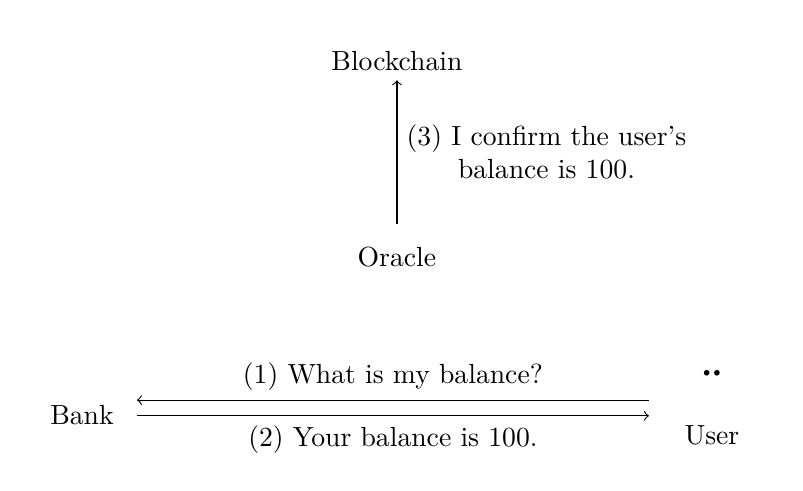
\begin{tikzpicture}
        \path (0, 0) node[align=center](Bank){{\Huge\texttt{ ^^^^^^0f0072 }} \\ Bank};
        \path (8, 0) node[align=center](User){{\Huge\texttt{ ^^^^^^0f0006 }} \\ User};
        \path (4, 2) node[align=center](Oracle){{\Huge\texttt{ ^^^^^^0f0ce5 }} \\ Oracle};
        \path (4, 4.5) node[align=center](Blockchain){{\Huge\texttt{ ^^^^^^0f0d1e }} \\ Blockchain};
        \draw[<-] ($(Bank.east) + (0, 0.1)$) -- ($(User.west) + (0, 0.1)$)
            node[midway, above] {(1) What is my balance?};
        \draw[->] ($(Bank.east) - (0, 0.1)$) -- ($(User.west) - (0, 0.1)$)
            node[midway, below] {(2) Your balance is 100.};
        \draw[->] (Oracle.north) -- (Blockchain.south)
            node[midway, right, align=center] {(3) I confirm the user's \\ balance is 100.};
    \end{tikzpicture}
    \end{center}
\end{frame}
% ---------------------------------------------------------------------------- %
\section{其他样式}
\subsection{列表样式}

\begin{frame}{列表样式}
\begin{quote}
    Do not use more than two levels of ``subitemizing''. beamer supports three levels, but you should not use that third level. Mostly, you should not even use the second one. Use good graphics instead.
    \cite{beamer-user-guide}
\end{quote}

\begin{columns}
    \begin{column}{0.5\linewidth}
        \begin{itemize}
            \item 第一层无序列表1.
            \item 第一层无序列表2.
            \begin{itemize}
                \item 第二层无序列表1.
                \item 第二层无序列表2.
                \begin{itemize}
                    \item 第三层无序列表1.
                    \item 第三层无序列表2.
                \end{itemize}
                \item 第二层无序列表3.
            \end{itemize}
            \item 第一层无序列表3.
        \end{itemize}
    \end{column}

    \begin{column}{0.5\linewidth}
        \begin{enumerate}
            \item 第一层有序列表1.
            \item 第一层有序列表2.
            \begin{enumerate}
                \item 第二层有序列表1.
                \item 第二层有序列表2.
                \begin{enumerate}
                    \item 第三层有序列表1.
                    \item 第三层有序列表2.
                \end{enumerate}
                \item 第二层有序列表3.
            \end{enumerate}
            \item 第一层有序列表3.
        \end{enumerate}
    \end{column}
\end{columns}
\end{frame}
% ---------------------------------------------------------------------------- %
\begin{frame}
    \begin{description}
        \item[描述列表1: ] 描述列表1的内容.
        \item[描述列表2: ] 描述列表2的内容.
        \item[描述列表3: ] 描述列表3的内容.
    \end{description}
\end{frame}
% ---------------------------------------------------------------------------- %
\subsection{块样式}

\begin{frame}\frametitle{块样式\alert{(待修改)}}

    \begin{block}{块标题}
        块内容
    \end{block}

    \begin{theorem}[Kummer, 1992]
        定理内容
    \end{theorem}

    \begin{proof}
        证明内容
    \end{proof}

    \begin{example}
        这是一个例子.
    \end{example}

\end{frame}
% ---------------------------------------------------------------------------- %
% ---------------------------------------------------------------------------- %
% ---------------------------------------------------------------------------- %

\section{待定}
\begin{frame}
    \sectionpage
\end{frame}
% ---------------------------------------------------------------------------- %
\section{其他}
\subsection{推荐资料}

\begin{frame}\frametitle{推荐资料}
LaTeX 教程:
    \begin{itemize}
        \item \fnlink{合集: 零基础入门 LaTeX}{https://space.bilibili.com/7240938/lists/52128}
    \end{itemize}
Beamer 教程:
    \begin{itemize}
        \item The beamer class User Guide: 在你的终端输入 \texttt{texdoc beamer} 查看.
    \end{itemize}
\end{frame}
% ---------------------------------------------------------------------------- %
\section{致谢}

\begin{frame}\frametitle{致谢}
字体:
\begin{itemize}
        \item \mdlink{LXGW Bright}{https://github.com/lxgw/LxgwBright}: 本文使用的 \textit{CJK 字体}.
        \item \mdlink{Sarasa Term SC Nerd Font}{https://github.com/laishulu/Sarasa-Term-SC-Nerd}: 本文使用的 \textit{英文正文字体}\  和 \textit{中英文 Mono 字体}.
        \item \mdlink{Fira Math}{https://github.com/firamath/firamath}: 本文使用的 \textit{数学字体}. 你可以在\mdlink{这里}{https://firamath.github.io/specimen.html}查看其支持的字符.
    \end{itemize}

beamer 主题:
\begin{itemize}
        \item \mdlink{Catppuccin for LaTeX Beamer}{https://github.com/atticus-sullivan/beamercolortheme} 
\includegraphics[height= 1.5 em,keepaspectratio]{./assets/figures/1544x1544_circle.png}
\end{itemize}

参考项目:
\begin{itemize}
        \item \mdlink{B\-站《Neovim 从入门到出门》系列教程}{https://space.bilibili.com/23686471/lists/5304627} 的 \mdlink{Slides}{https://github.com/Jacky-Lzx/nvim.tutorial.slides}.
\end{itemize}
\end{frame}
% ---------------------------------------------------------------------------- %
\section{参考文献}

\begin{frame}\frametitle{参考文献}
    \begin{quote}
        You can use the bibliography environment and the \texttt{\textbackslash cite} commands of LATEX in a beamer presentation. You will typically have to typeset your bibliography items partly ``by hand''. Nevertheless, you can use bibtex to create a ``first approximation'' of the bibliography. Copy the content of the file main.bbl into your presentation.
        \cite{beamer-user-guide}
    \end{quote}

    % \bibliographystyle{plain}
    % \bibliography{ref}
    \begin{thebibliography}{1}

    \bibitem[Tantau, 2025]{beamer-user-guide}
    Till Tantau{,} Joseph Wright{,}~Vedran Miletić.
    \newblock The beamer class, 2025.

    \end{thebibliography}
\end{frame}



\end{document}